\documentclass[a4paper,10pt]{article}
\usepackage[utf8]{inputenc}
\usepackage[spanish]{babel}
\usepackage{fancyhdr}
\usepackage{multicol}
\usepackage{geometry}
\usepackage{graphicx}
\usepackage{amsmath}
\usepackage{hyperref}
\geometry{a4paper, portrait, margin=1in}

\pagestyle{fancy}
\fancyhf{}
\fancyhead[L]{\textbf{Estad\'istica Computacional}}
\fancyhead[R]{Universidad Nacional del Altiplano - FINESI}
\fancyfoot[C]{\thepage}

\begin{document}

\begin{center}
    \textbf{\Large Universidad Nacional del Altiplano - FINESI} \\[1em]
    \textbf{\large Estadística Computacional} \\[1em]
    
    \textbf{Docente:} Ing. Torres Cruz Fred \\
    \textbf{Estudiante:} Mamani Huatta Cliver Daniel \\
    \textbf{Código:} 231211 \\[2em]
    
    \textbf{Fecha:} Puno, 5 de mayo de 2025
\end{center}

\vspace{1em} 


\section*{Interfaz Visual del M\'etodo de Soluci\'on}

\subsection*{1. Descripci\'on del Problema}
Se ha implementado una aplicaci\'on para resolver un problema de optimizaci\'on lineal. Este tipo de problema busca maximizar o minimizar una funci\'on lineal sujeta a restricciones tambi\'en lineales.

En nuestro caso, el problema tiene la forma:
\begin{itemize}
  \item Maximizar $z = a \cdot x + b \cdot y$
  \item Sujeto a:
  \begin{itemize}
    \item $x + y \leq c$ (restricci\'on combinada)
    \item $x \leq x_{\text{m\'ax}}$ (l\'imite superior de x)
    \item $y \leq y_{\text{m\'ax}}$ (l\'imite superior de y)
    \item $x, y \geq 0$ (no negatividad)
  \end{itemize}
\end{itemize}
Este modelo puede representar, por ejemplo, la distribuci\'on \"optima de recursos entre dos actividades.

\subsection*{2. Framework Utilizado: Flask}
\begin{itemize}
  \item Flask es un microframework web en Python.
  \item Es liviano, sencillo y muy flexible, ideal para proyectos peque\~nos y prototipos r\'apidos.
  \item Permite manejar formularios, procesar entradas del usuario y mostrar resultados din\'amicos.
  \item Fue elegido por su facilidad de integraci\'on con HTML y su curva de aprendizaje baja.
  \item El archivo principal se llama \texttt{app.py} y define las rutas, la l\'ogica del c\'alculo y el renderizado de resultados.
\end{itemize}

\subsection*{3. Interfaz Visual Desarrollada}
\begin{itemize}
  \item Se dise\~n\'o una p\'agina web con HTML que permite al usuario ingresar los valores de entrada:
  \begin{itemize}
    \item Coeficientes de la funci\'on objetivo: $a$ y $b$
    \item L\'imite de la restricci\'on combinada: $c$
    \item Valores m\'aximos permitidos para $x$ y $y$
  \end{itemize}
  \item Al enviar el formulario, Flask procesa los datos y calcula el valor m\'aximo de $z$ y el punto $(x, y)$ donde se alcanza.
  \item La soluci\'on se presenta de forma clara directamente en la misma p\'agina.
\end{itemize}

\begin{center}
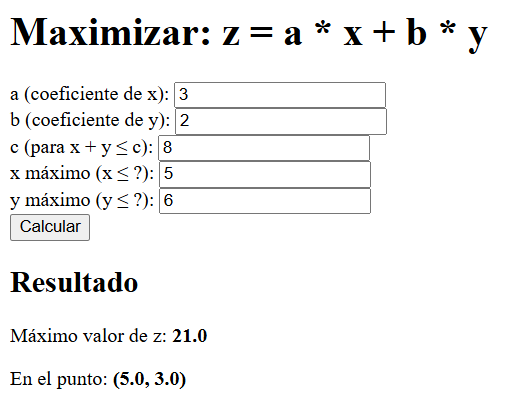
\includegraphics[width=0.8\textwidth]{ejemplo_interfaz.png}
\end{center}

\subsection*{4. Ejemplo de C\'alculo}
\begin{itemize}
  \item Supongamos los siguientes valores:
  \begin{itemize}
    \item $a = 3$, $b = 2$, $c = 8$, $x_{\text{m\'ax}} = 5$, $y_{\text{m\'ax}} = 6$
  \end{itemize}
  \item El programa calcula los v\'ertices factibles de la regi\'on definida por las restricciones.
  \item Se eval\'ua la funci\'on objetivo $z = 3x + 2y$ en cada v\'ertice.
  \item Se selecciona el punto donde $z$ alcanza su m\'aximo valor.
  \item Resultado:
  \begin{itemize}
    \item M\'aximo valor de $z$: \textbf{21}
    \item En el punto $(5, 3)$
  \end{itemize}
\end{itemize}

\subsection*{5. Conclusi\'on}
\begin{itemize}
  \item La implementaci\'on con Flask permiti\'o desarrollar una interfaz funcional y sencilla para resolver problemas de optimizaci\'on lineal.
  \item Se logra integrar Python con HTML para brindar una experiencia de usuario interactiva.
  \item El m\'etodo es replicable y extensible a m\'as restricciones o variables si se desea mejorar.
  \item Este proyecto es un ejemplo claro de c\'omo la estad\'istica computacional se aplica en la resoluci\'on de problemas reales.
\end{itemize}

\end{document}